% Appendix B

\chapter{Distribuições Temporais da Validação Externa do Relógio}
\label{AppendixB}

Este apêndice apresenta as distribuições temporais complementares das previsões obtidas durante a validação externa dos modelos de agrupamento treinados com dados do relógio Empatica EmbracePlus. São apresentados os resultados das configurações que não foram incluídas no corpo principal da tese, considerando três situações experimentais: trabalho em computador, atividade física e sono.

Por razões de legibilidade, no corpo principal da tese foram apresentadas apenas as distribuições temporais do GMM com dados originais. As figuras seguintes complementam essa análise e documentam o comportamento do GMM com janelas temporais de 10 minutos, do Clustering Hierárquico com dados originais e do Clustering Hierárquico com janelas temporais de 10 minutos. Em cada conjunto, as imagens correspondem, respetivamente, ao trabalho em computador, à atividade física e ao sono.

Os resultados encontram-se apresentados pela seguinte ordem:
\begin{enumerate}
    \item \textbf{GMM Restrito com dados originais ($k=4$):} modelo de GMM configurado para representar os dados em apenas quatro clusters. Imagens: a) trabalho em computador; b) atividade física; c) sono (Figura~\ref{fig:apendice_gmm_restrito}).
    \item \textbf{GMM com janelas de 10 minutos ($k=5$):} modelo de GMM aplicado a janelas temporais de 10 minutos, com cinco clusters, selecionados pelo BIC mínimo. Imagens: a) trabalho em computador; b) atividade física; c) sono (Figura~\ref{fig:apendice_gmm_janelas}).
    \item \textbf{Clustering Hierárquico com dados originais ($k=5$):} modelo de agrupamento hierárquico aplicado aos dados originais, com cinco clusters. Imagens: a) trabalho em computador; b) atividade física; c) sono (Figura~\ref{fig:apendice_hier_original}).
    \item \textbf{Clustering Hierárquico com janelas de 10 minutos ($k=5$):} modelo de agrupamento hierárquico aplicado a janelas temporais de 10 minutos, com cinco clusters. Imagens: a) trabalho em computador; b) atividade física; c) sono (Figura~\ref{fig:apendice_hier_janelas}).
\end{enumerate}

\section{GMM Restrito com Dados Originais ($k=4$)}
\label{sec:apendice_gmm_restrito}

\begin{figure}[H]
\centering
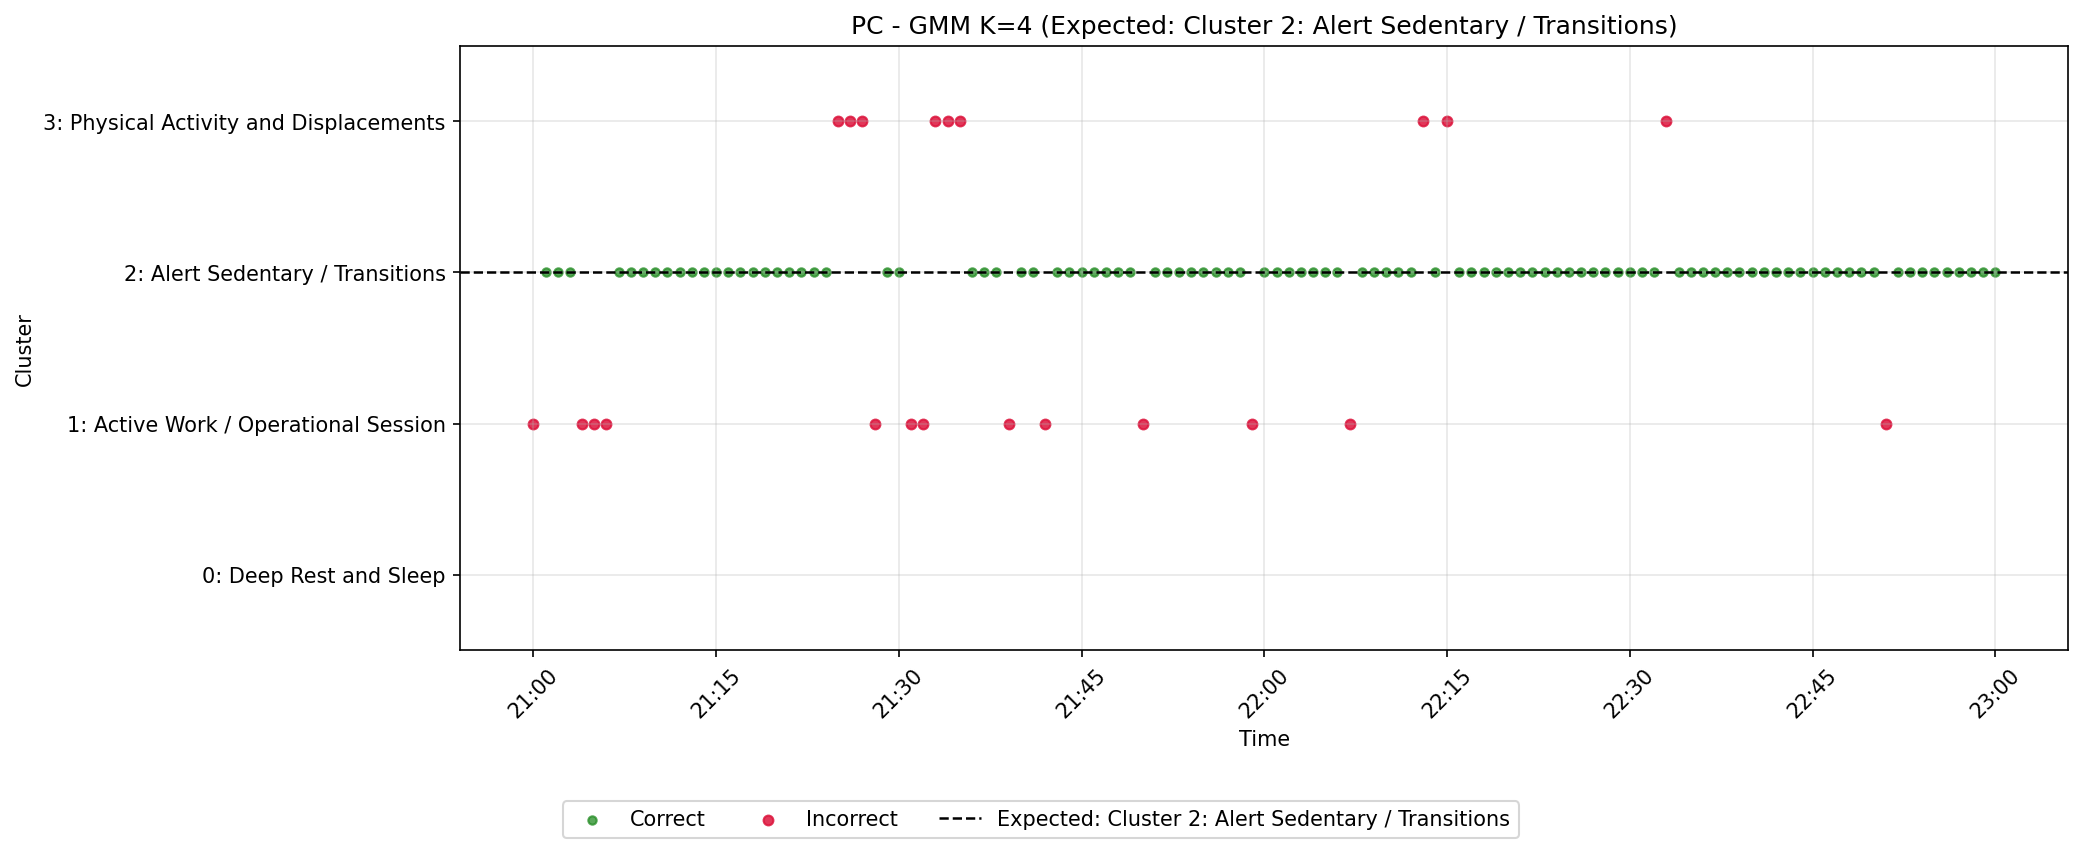
\includegraphics[width=0.95\textwidth]{ch4/assets/validacao_gmm_restrito_trabalho.png}
\centerline{(a) Trabalho em computador}
\par\vspace{0.5em}
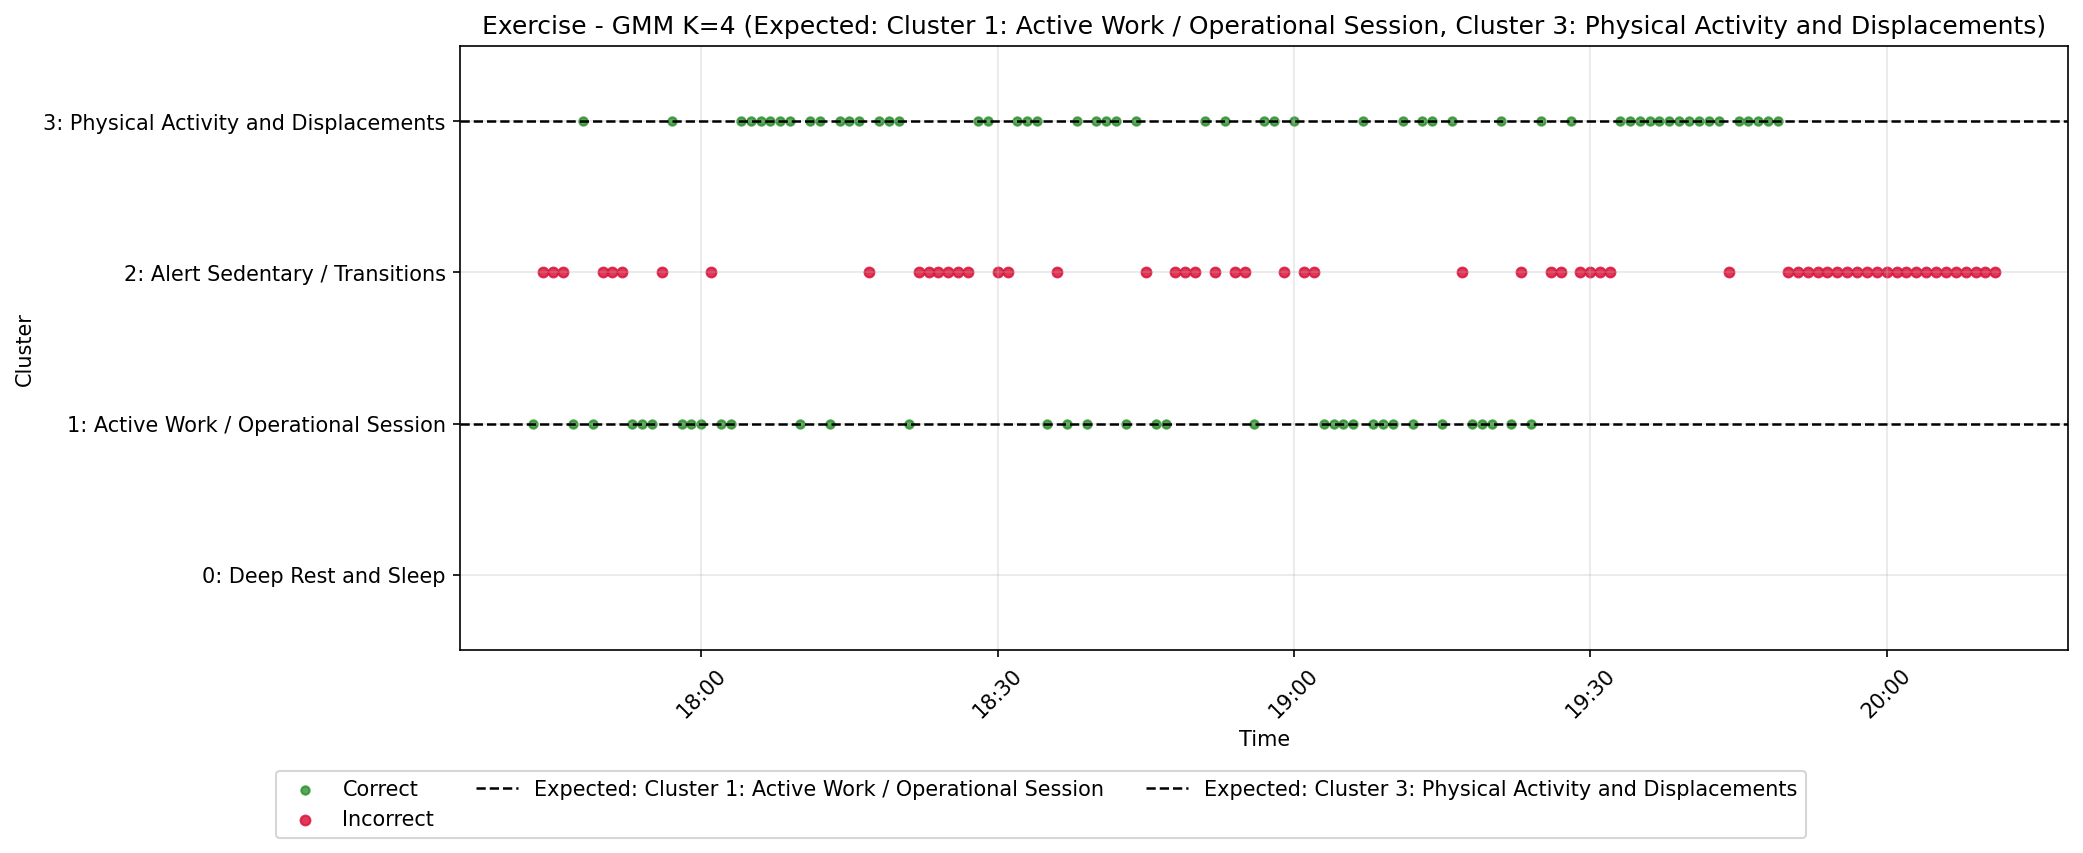
\includegraphics[width=0.95\textwidth]{ch4/assets/validacao_gmm_restrito_atividade_fisica.png}
\centerline{(b) Atividade física}
\par\vspace{0.5em}
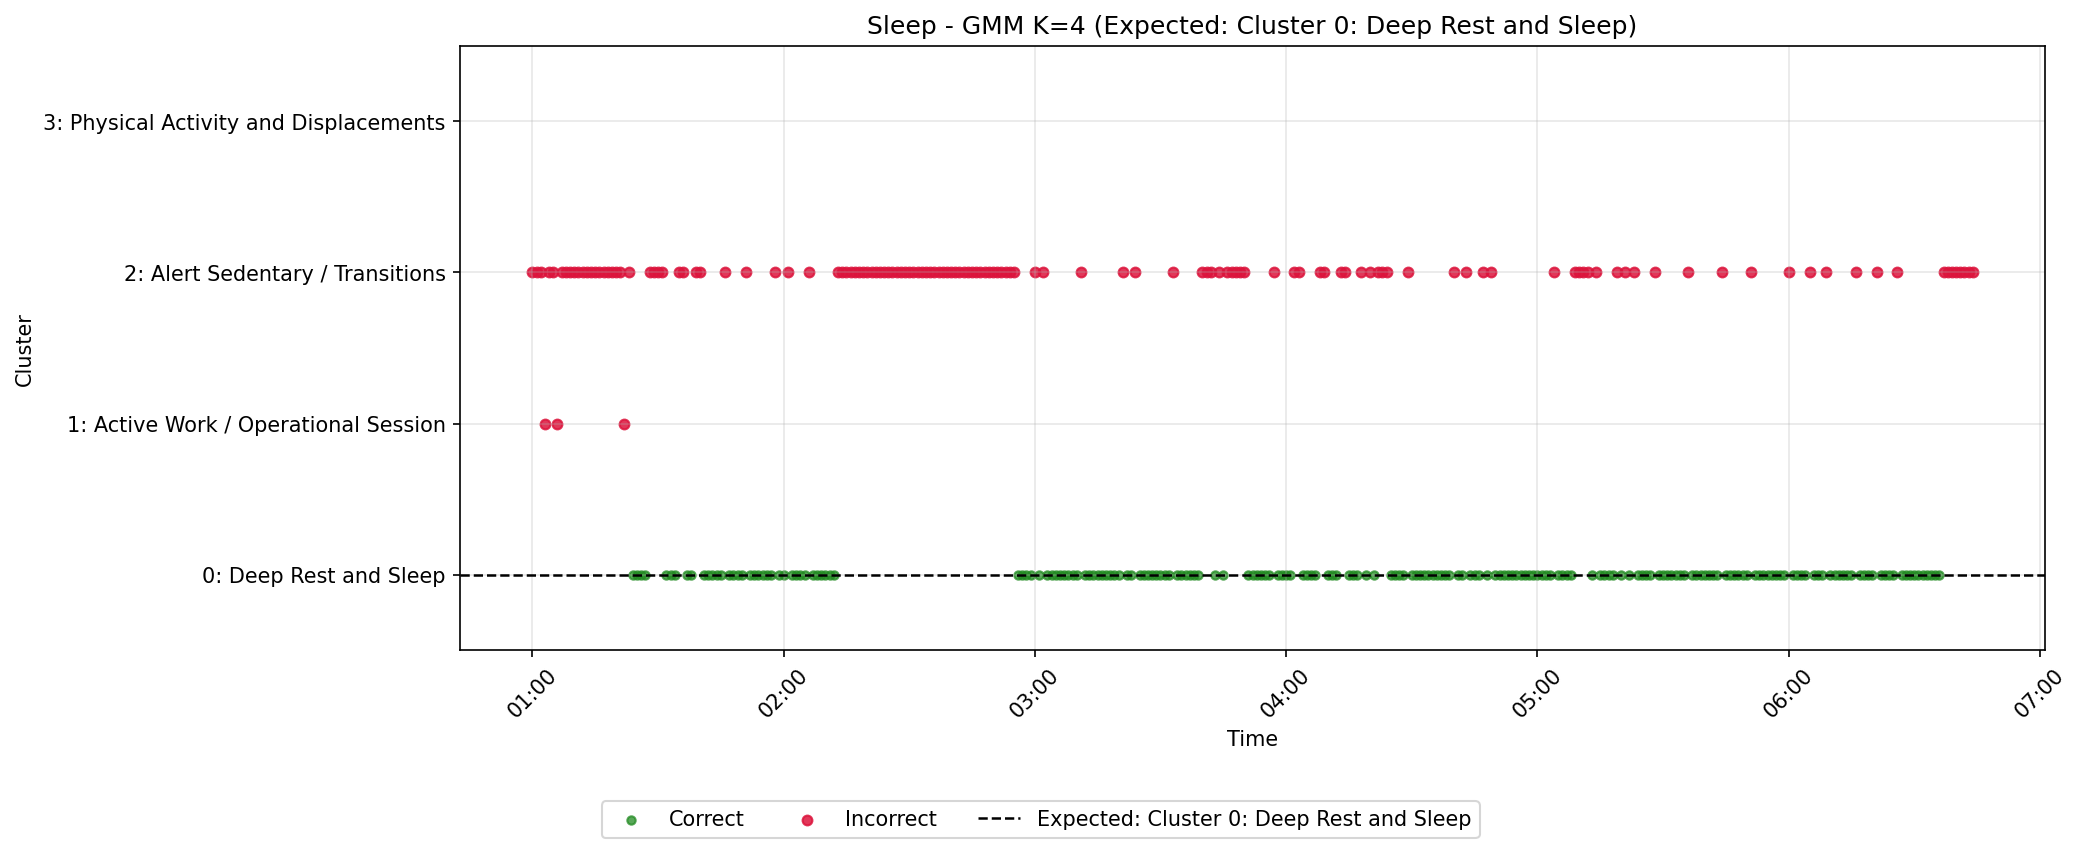
\includegraphics[width=0.95\textwidth]{ch4/assets/validacao_gmm_restrito_sono.png}
\centerline{(c) Sono}
\caption{Distribuição temporal das previsões do GMM Restrito com dados originais ($k=4$) durante as três atividades experimentais.}
\label{fig:apendice_gmm_restrito}
\end{figure}

\section{GMM com Janelas de 10 Minutos ($k=5$)}
\label{sec:apendice_gmm_janelas}

\begin{figure}[H]
\centering
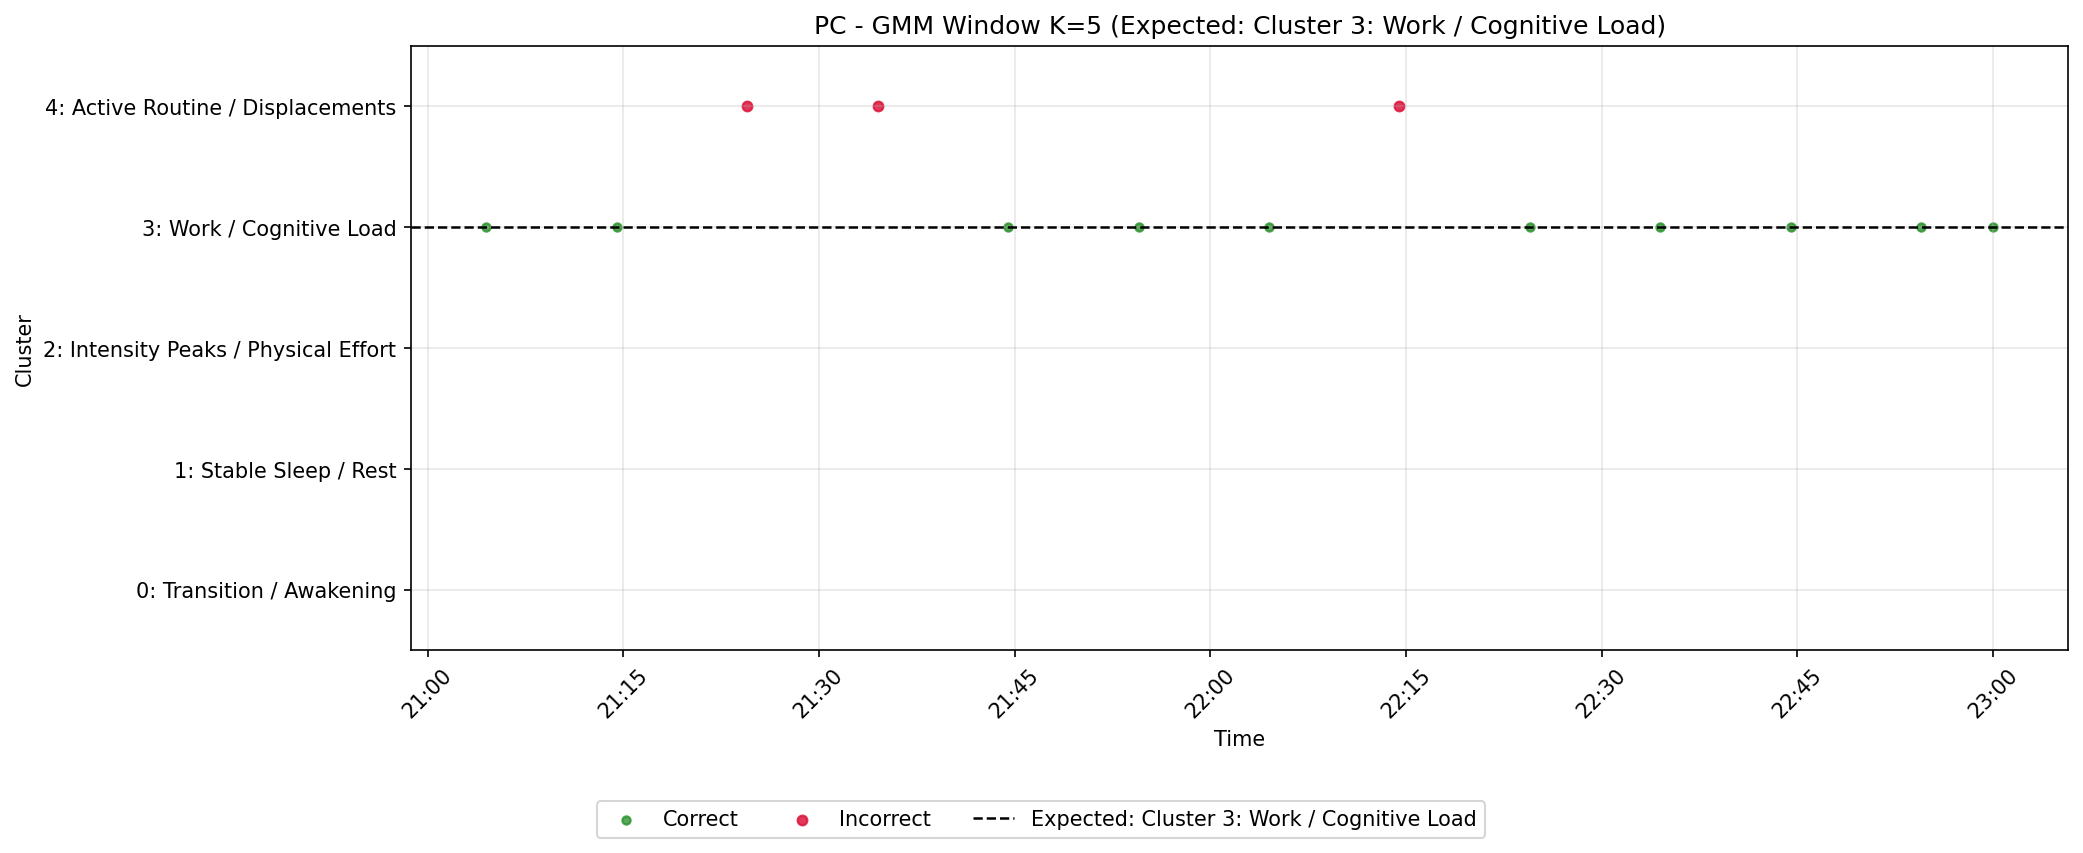
\includegraphics[width=0.95\textwidth]{ch4/assets/validacao_gmm_janelas_trabalho.png}
\centerline{(a) Trabalho em computador}
\par\vspace{0.5em}
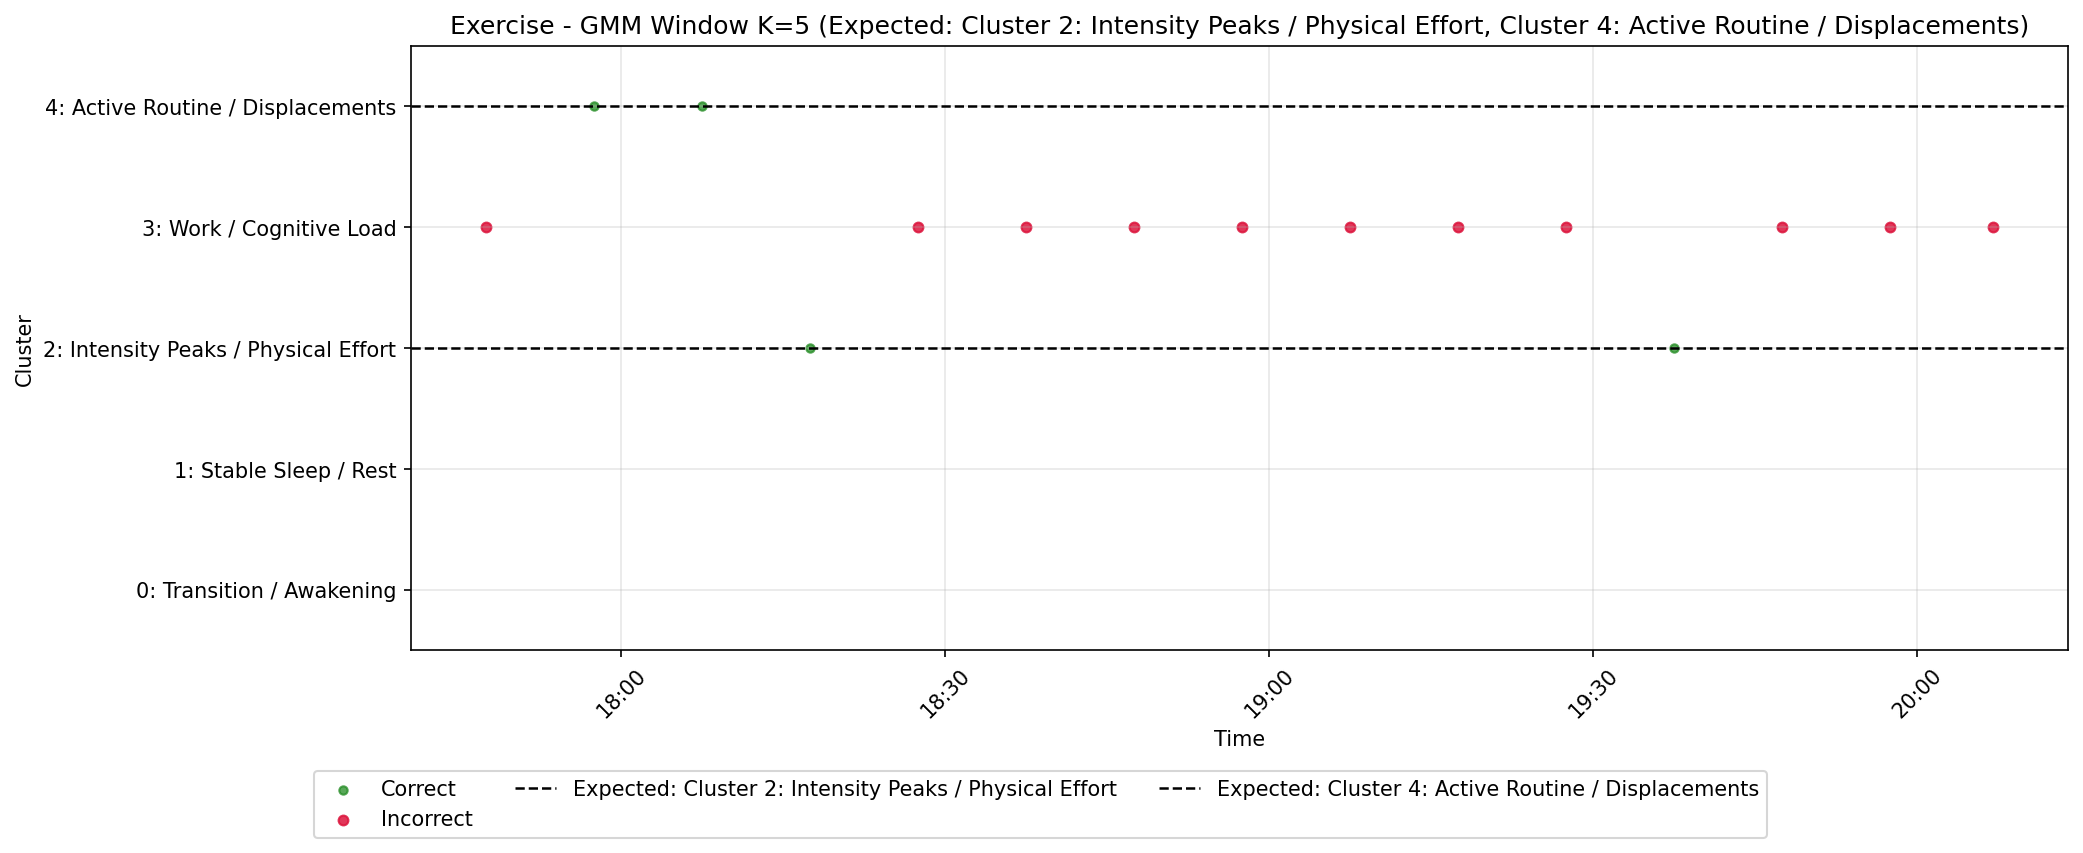
\includegraphics[width=0.95\textwidth]{ch4/assets/validacao_gmm_janelas_atividade_fisica.png}
\centerline{(b) Atividade física}
\par\vspace{0.5em}
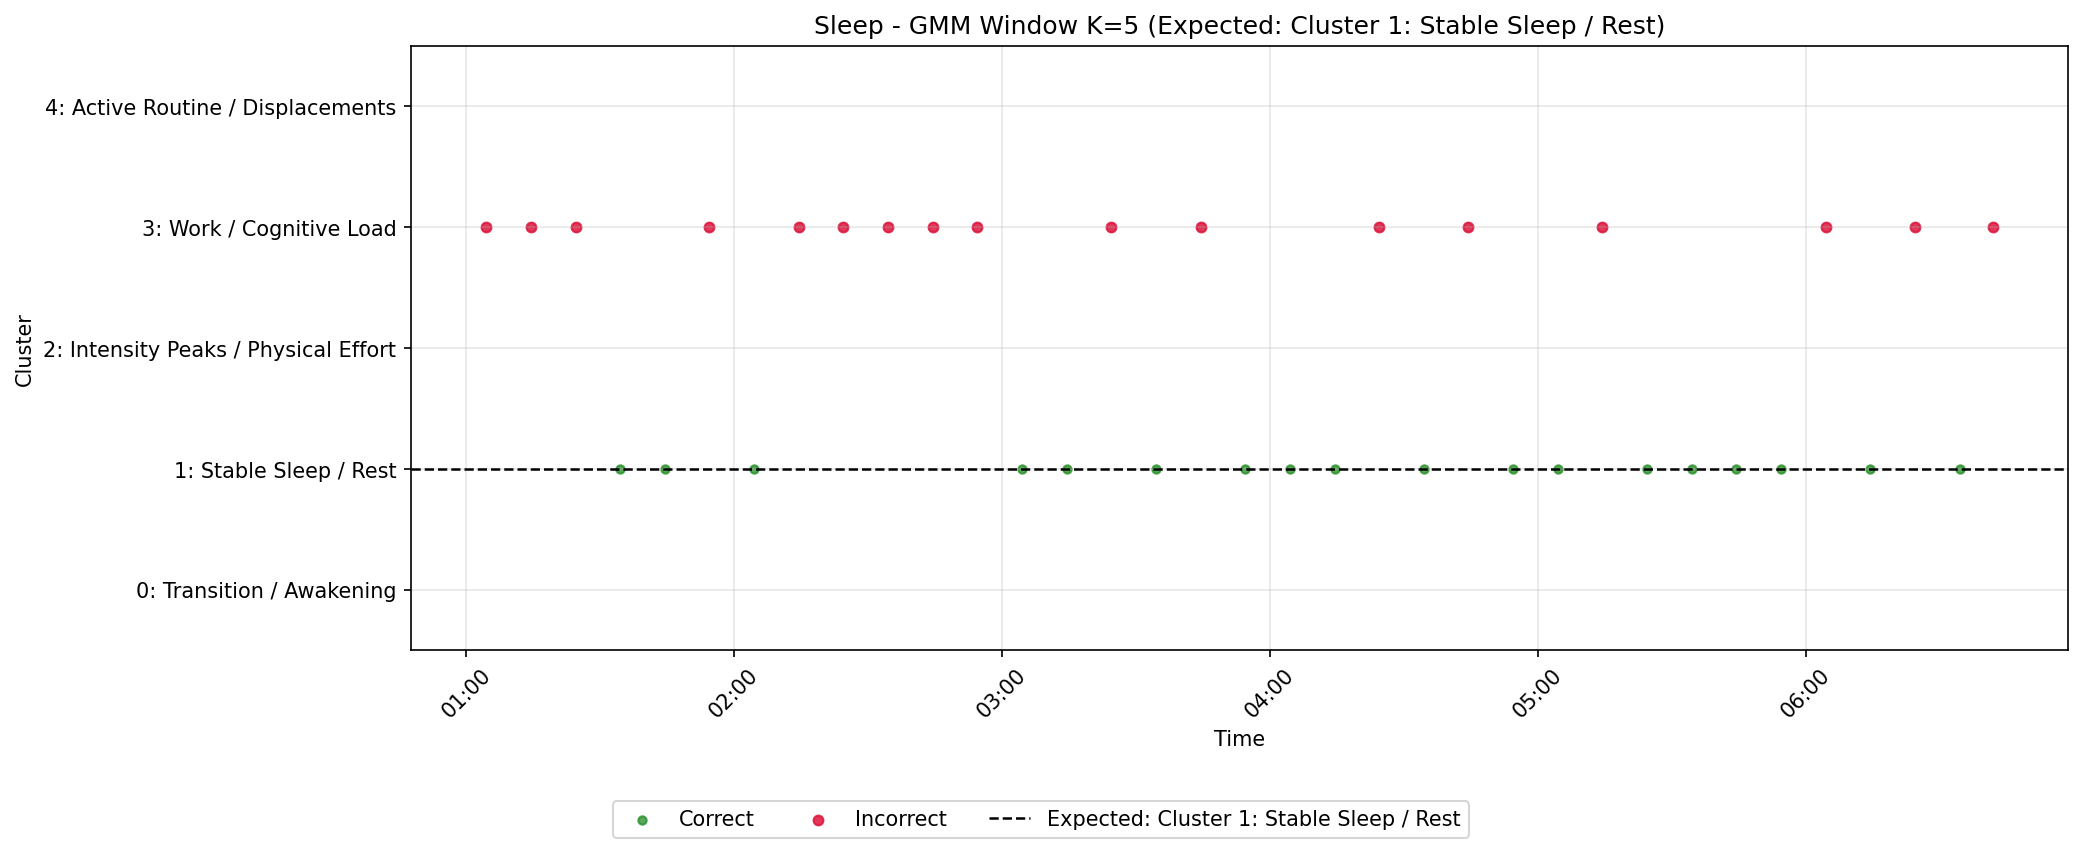
\includegraphics[width=0.95\textwidth]{ch4/assets/validacao_gmm_janelas_sono.png}
\centerline{(c) Sono}
\caption{Distribuição temporal das previsões do GMM com janelas de 10 minutos ($k=5$) durante as três atividades experimentais.}
\label{fig:apendice_gmm_janelas}
\end{figure}

\section{Clustering Hierárquico com Dados Originais ($k=5$)}
\label{sec:apendice_hier_original}

\begin{figure}[H]
\centering
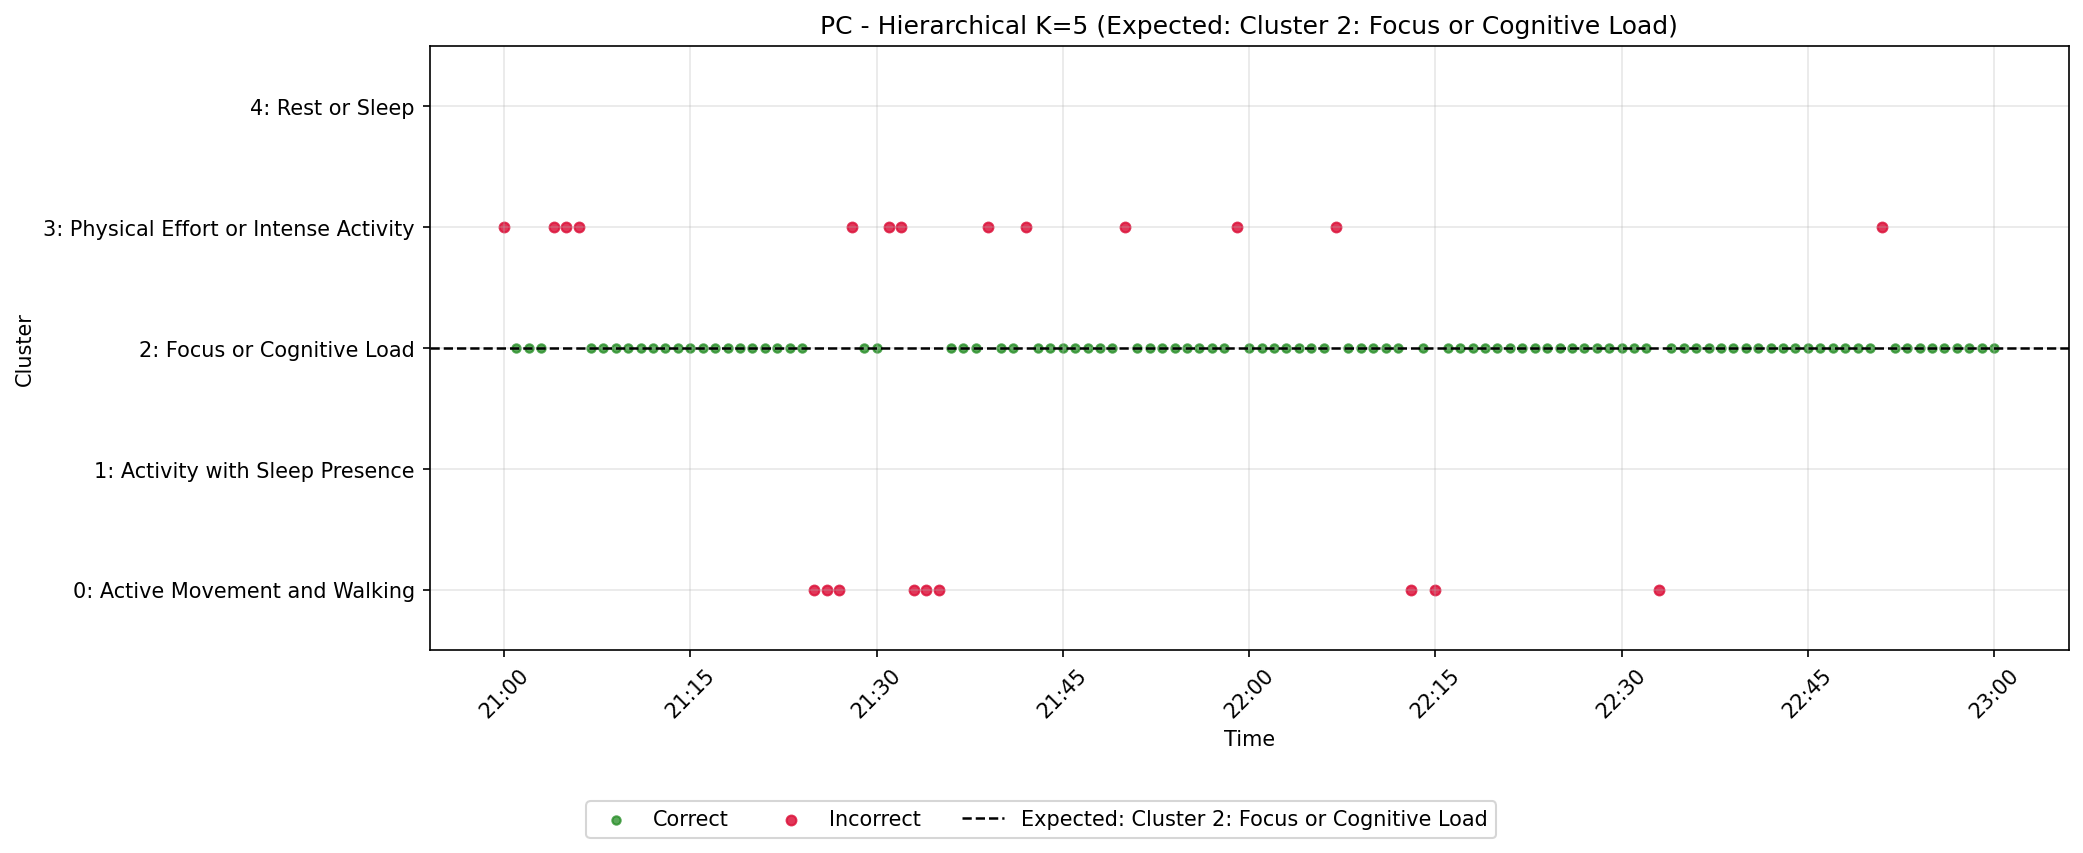
\includegraphics[width=0.95\textwidth]{ch4/assets/validacao_hierarquico_original_trabalho.png}
\centerline{(a) Trabalho em computador}
\par\vspace{0.5em}
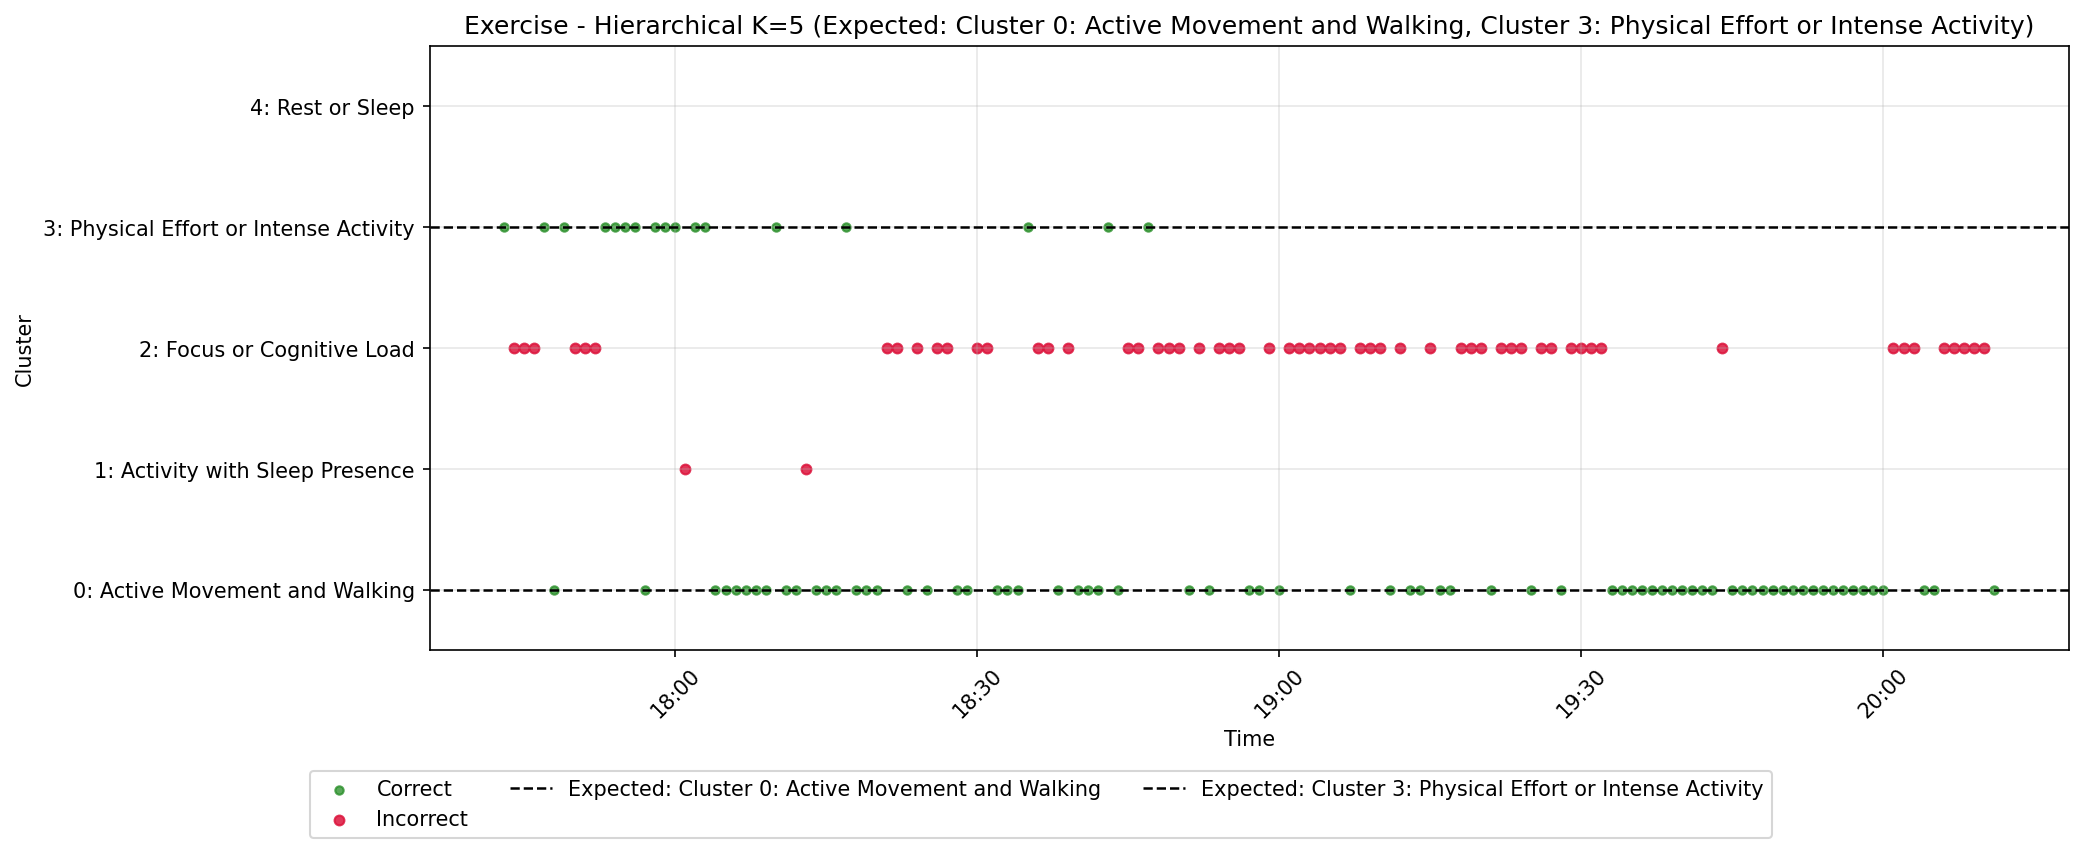
\includegraphics[width=0.95\textwidth]{ch4/assets/validacao_hierarquico_original_atividade_fisica.png}
\centerline{(b) Atividade física}
\par\vspace{0.5em}
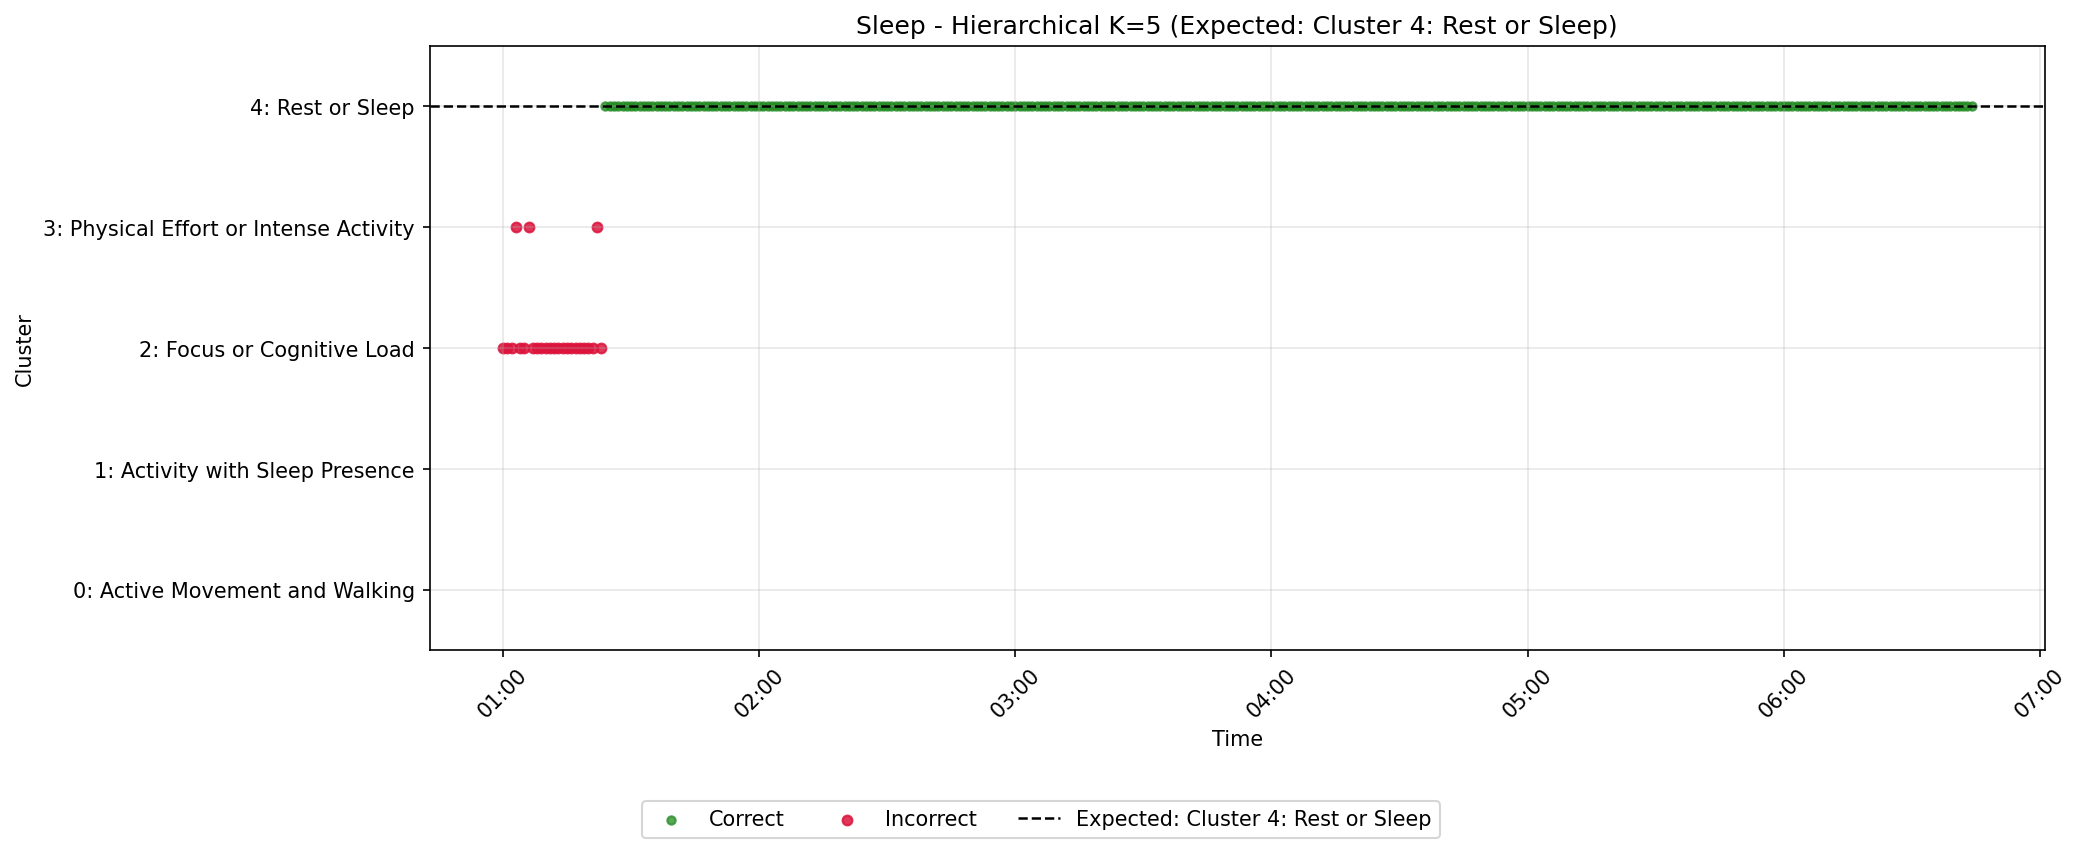
\includegraphics[width=0.95\textwidth]{ch4/assets/validacao_hierarquico_original_sono.png}
\centerline{(c) Sono}
\caption{Distribuição temporal das previsões do Clustering Hierárquico com dados originais ($k=5$) durante as três atividades experimentais.}
\label{fig:apendice_hier_original}
\end{figure}

\section{Clustering Hierárquico com Janelas de 10 Minutos ($k=5$)}
\label{sec:apendice_hier_janelas}

\begin{figure}[H]
\centering
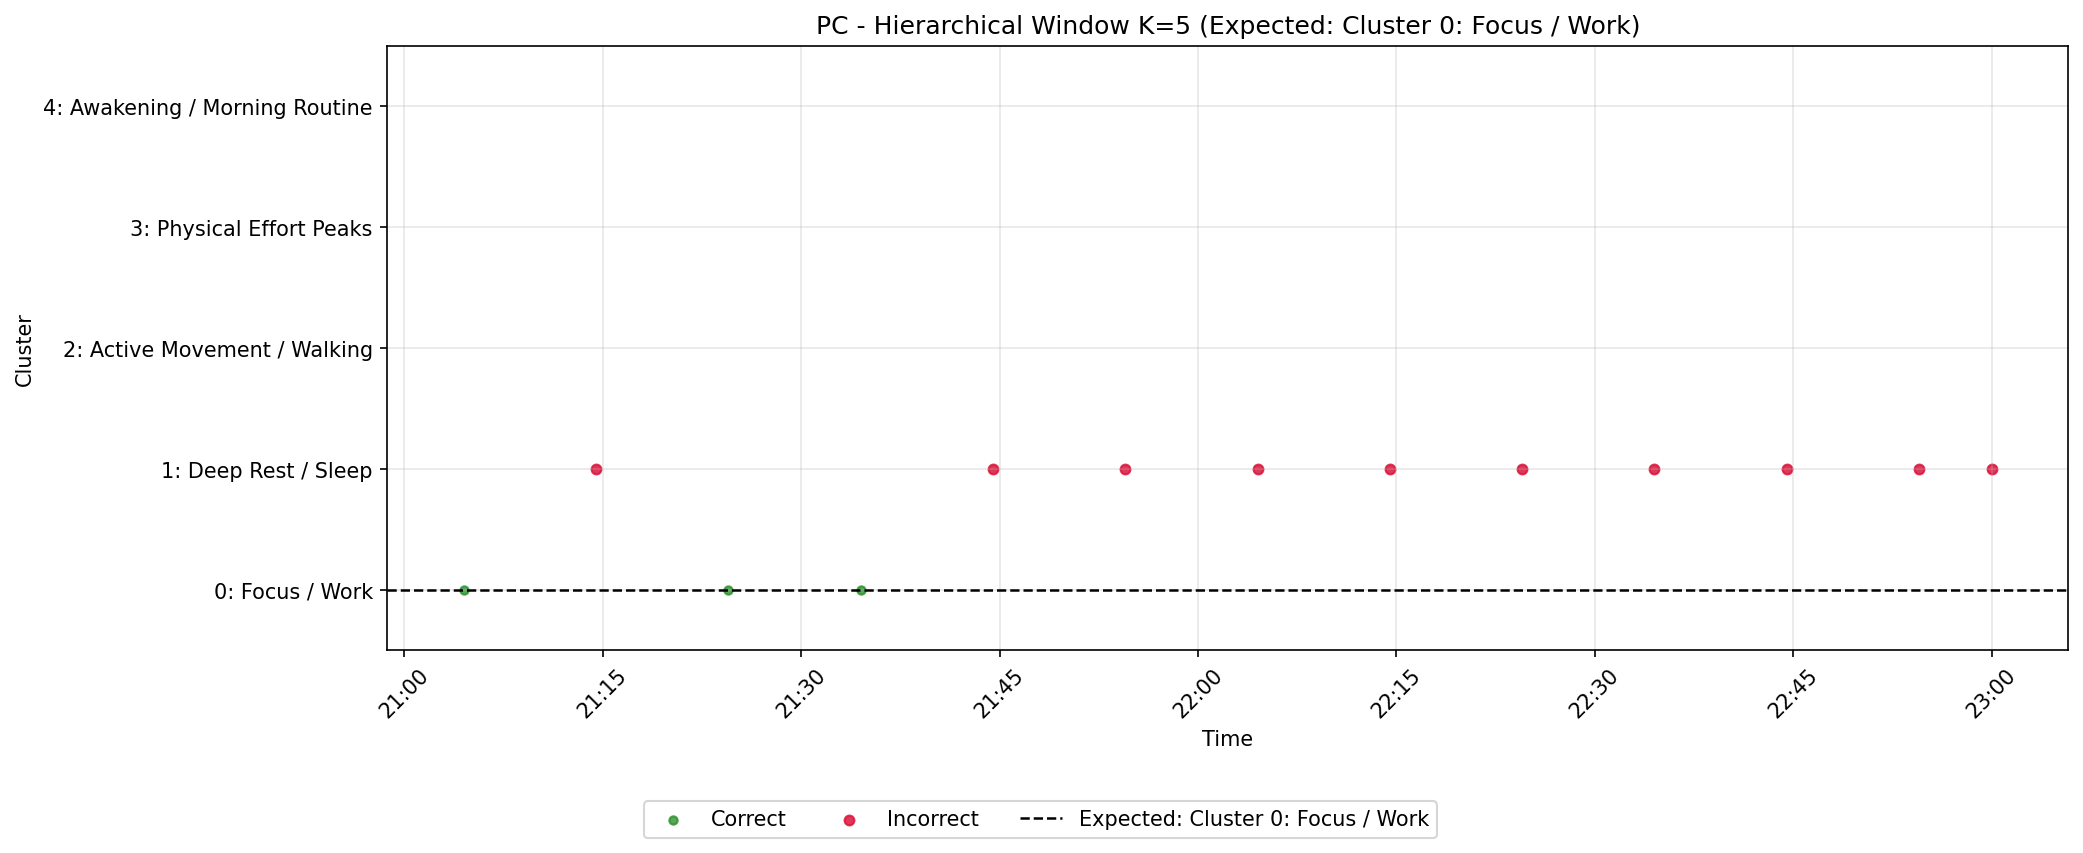
\includegraphics[width=0.95\textwidth]{ch4/assets/validacao_hierarquico_janelas_trabalho.png}
\centerline{(a) Trabalho em computador}
\par\vspace{0.5em}
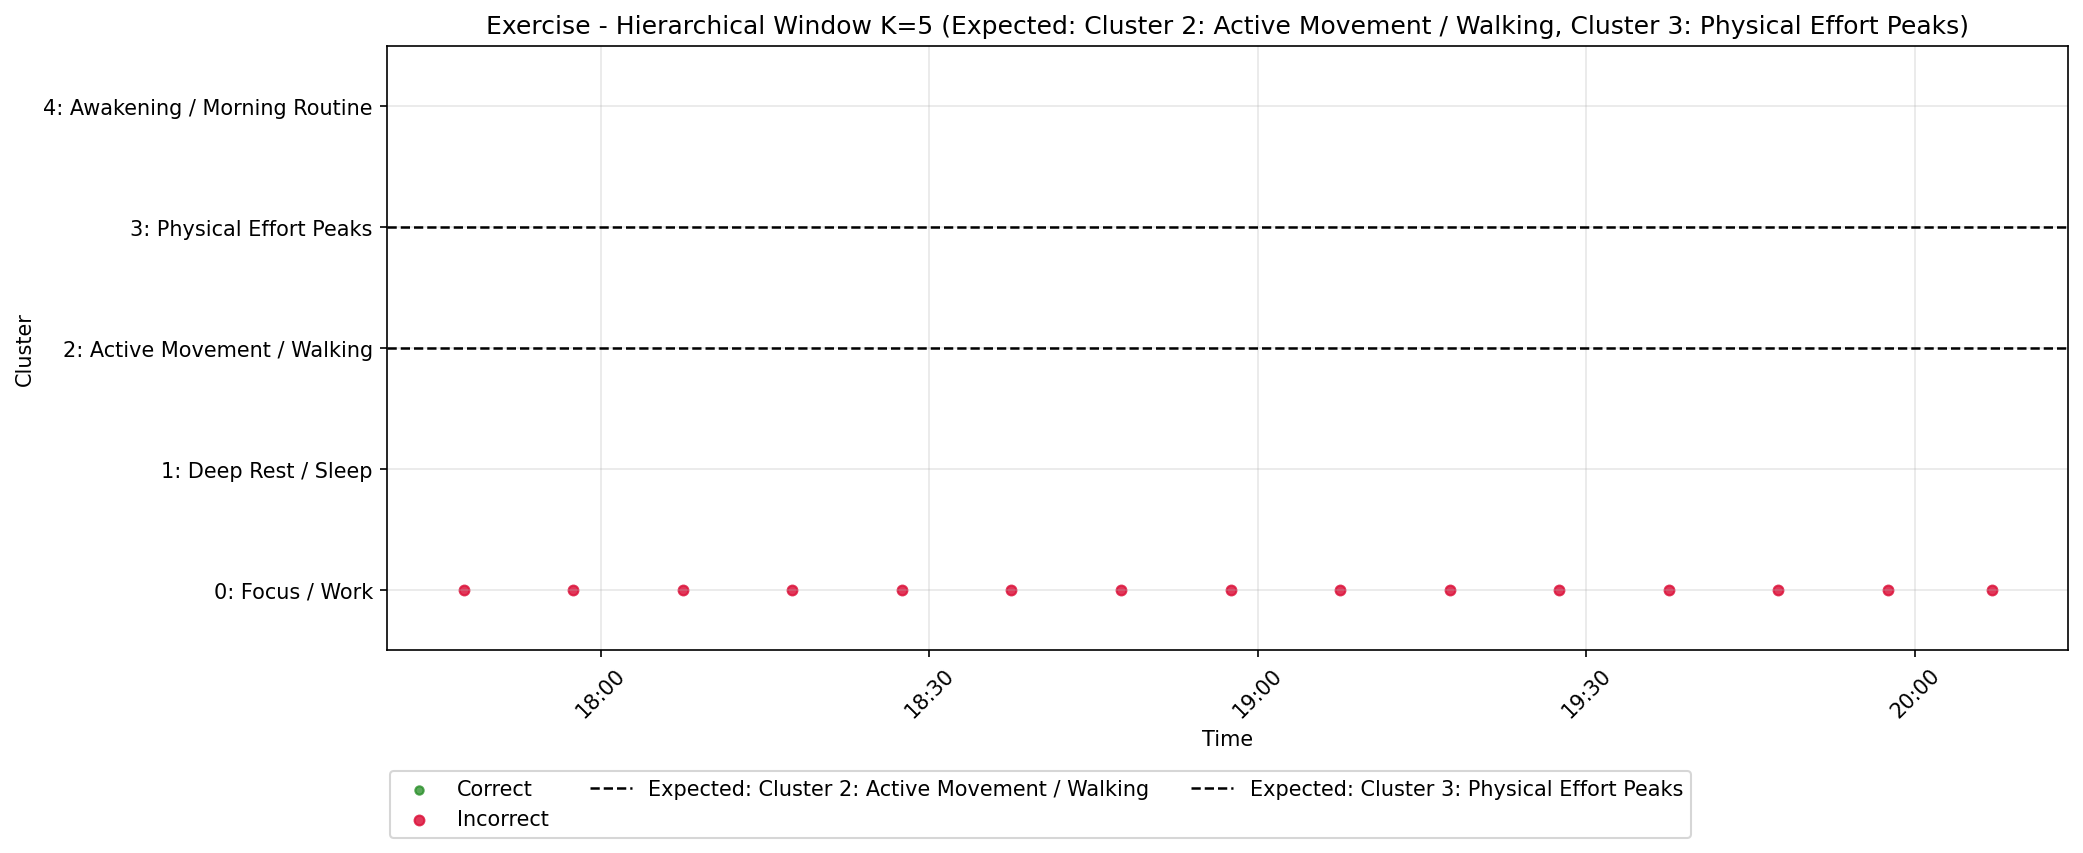
\includegraphics[width=0.95\textwidth]{ch4/assets/validacao_hierarquico_janelas_atividade_fisica.png}
\centerline{(b) Atividade física}
\par\vspace{0.5em}
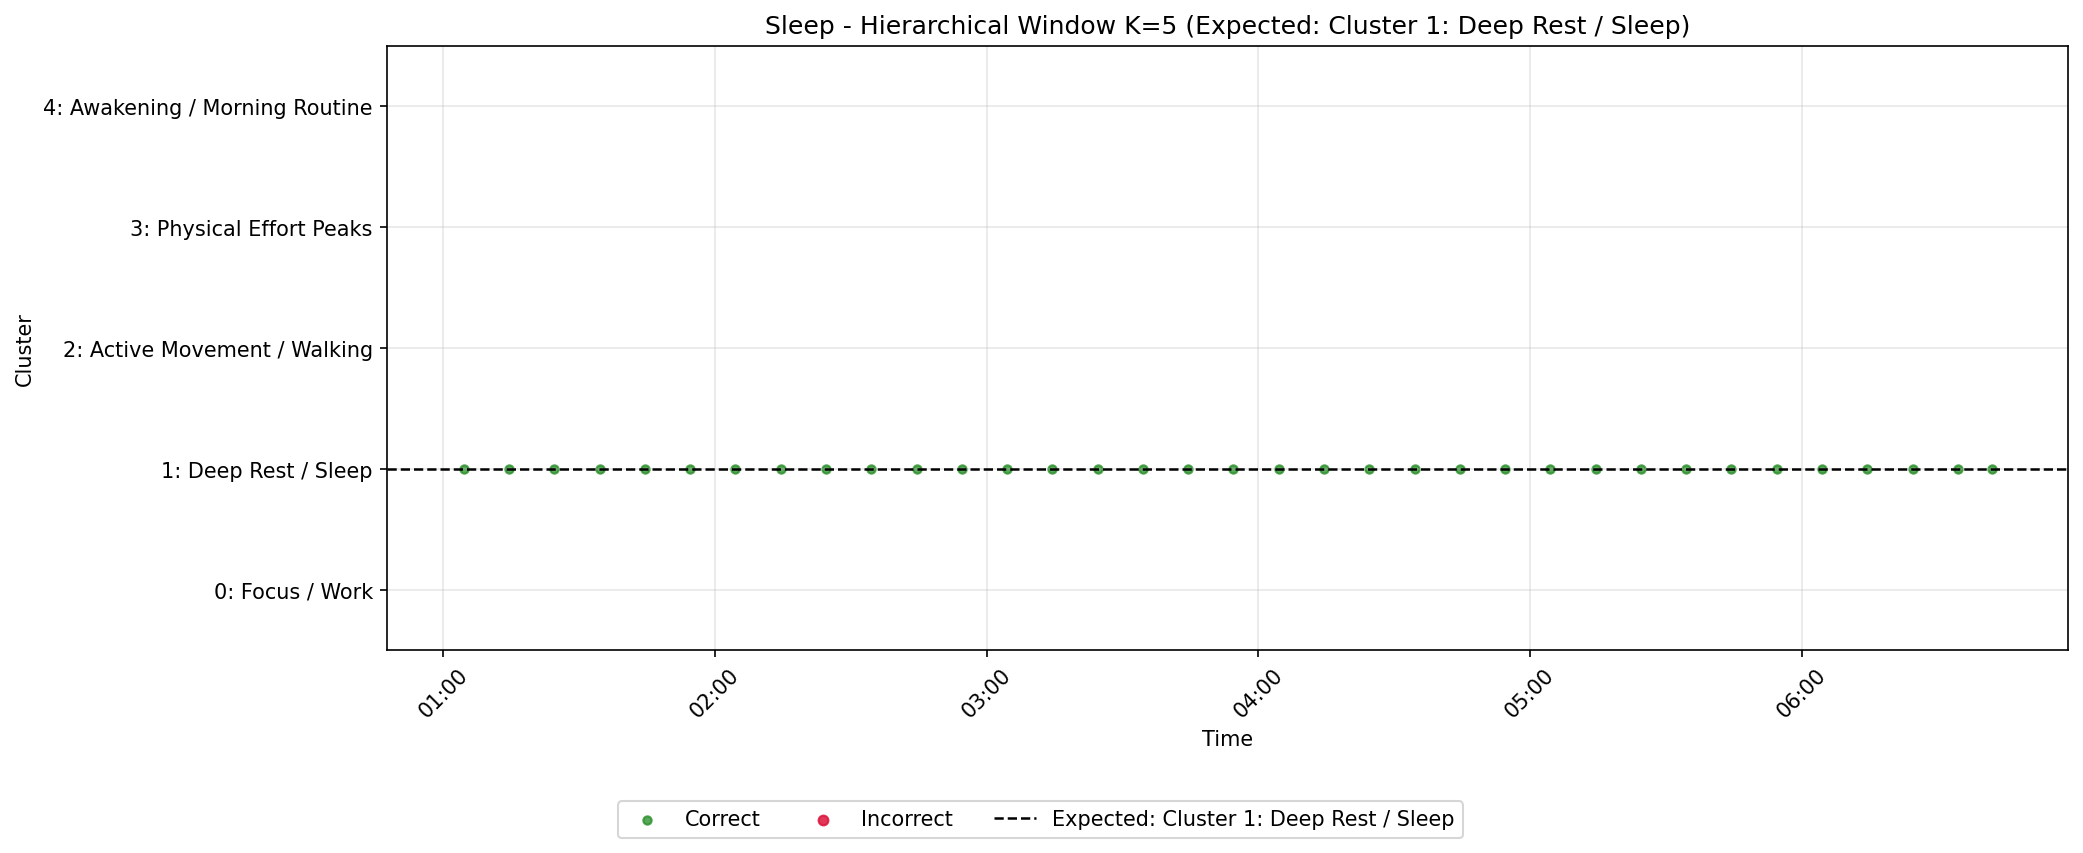
\includegraphics[width=0.95\textwidth]{ch4/assets/validacao_hierarquico_janelas_sono.png}
\centerline{(c) Sono}
\caption{Distribuição temporal das previsões do Clustering Hierárquico com janelas de 10 minutos ($k=5$) durante as três atividades experimentais.}
\label{fig:apendice_hier_janelas}
\end{figure}
